\documentclass[a4paper,twoside,11pt, fleqn]{article}
\usepackage{a4wide,graphicx,fancyhdr,amsmath,amssymb}
\usepackage{listings}
\usepackage{color}
\usepackage{dirtree}
\usepackage{subcaption}

%matlab 
\usepackage[]{mcode}

%----------------------- Macros and Definitions --------------------------

\setlength\headheight{20pt}
\addtolength\topmargin{-10pt}
\addtolength\footskip{20pt}

\newcommand{\N}{\mathbb{N}}
\newcommand{\ch}{\mathcal{CH}}

\newcommand{\solution}[1]{\noindent{\bf Solution to Exercise #1:}}

\fancypagestyle{plain}{%
\fancyhf{}
\fancyhead[LO,RE]{\sffamily\bfseries\large technische universiteit eindhoven}
\fancyhead[RO,LE]{\sffamily\bfseries\large 2IN35 VLSI}
\fancyfoot[LO,RE]{\sffamily\bfseries\large department of mathematics and computer science}
\fancyfoot[RO,LE]{\sffamily\bfseries\thepage}
\renewcommand{\headrulewidth}{0pt}
\renewcommand{\footrulewidth}{0pt}
}

\pagestyle{fancy}
\fancyhf{}
\fancyhead[RO,LE]{\sffamily\bfseries\large technische universiteit eindhoven}
\fancyhead[LO,RE]{\sffamily\bfseries\large 2IN35 VLSI}
\fancyfoot[LO,RE]{\sffamily\bfseries\large department of mathematics and computer science}
\fancyfoot[RO,LE]{\sffamily\bfseries\thepage}
\renewcommand{\headrulewidth}{1pt}
\renewcommand{\footrulewidth}{0pt}

\def\addsquare#1{\tikz\node[draw]{#1};} 

%-------------------------------- Title ----------------------------------

\title{\vspace{-\baselineskip}\sffamily\bfseries Assignment 4}
\author{
	Rick Veens \qquad Studentno: 0912292\\
	\texttt{r.veens@student.tue.nl}
	\and
	Barry de Bruin \qquad Studentno: 0919605\\
	\texttt{e.d.bruin@student.tue.nl}
	\and
	\texttt{Group 7}
}

\date{\today}

\setlength\parindent{0pt}

%--------------------------------- Text ----------------------------------

\begin{document}
\maketitle
\newpage

\tableofcontents

\newpage
\section{Inline questions}
\subsection{Inline question 1}
The theoretical bound would be one cycle per output sample. The maximum number of streams would then be:\\

$max_{\# streams} = \dfrac{system\_frequency \cdot sample\_frequency}{\frac{cycles}{sample}} = \dfrac{100MHz \cdot 48KHz}{1} \approx 2083$ streams\\

\subsection{Inline question 2}
We waste two cycles to shift in one sample of data. Then we also use one cycle to make sure that the output acknowledge is received, and we use one cycle to calculate a sample. If we re-use the samples (due to upsampling), we will not use the two cycles to process the input.\\

Every 147 input samples, we produce 160 output samples. If we assume that the acknowledgement of input and output occurs the very next cycle after requesting (which is probably not very likely), the amount of cycles required to produce 160 samples is:
\begin{align*}
amount\_of\_cycles &= 147\cdot (2 + 1 + 1) + (160-147)\cdot (1  + 1 )\\
&= 588 + 26\\
&= 614
\end{align*}

This will result in: $\frac{614}{160} \approx 4$ cycles per sample. 

\subsection{Inline question 3}
Since we have 2083 clock cycles available, to produce all samples of one stream, and our design needs approximately 4 cycles to produce one output, our maximum output stream number is limited to $\frac{2083}{4} \approx 521$ streams.

\newpage
\section{System architecture}
Figure one shows the global architecture of the FIR filter. 
\begin{figure}[h]
	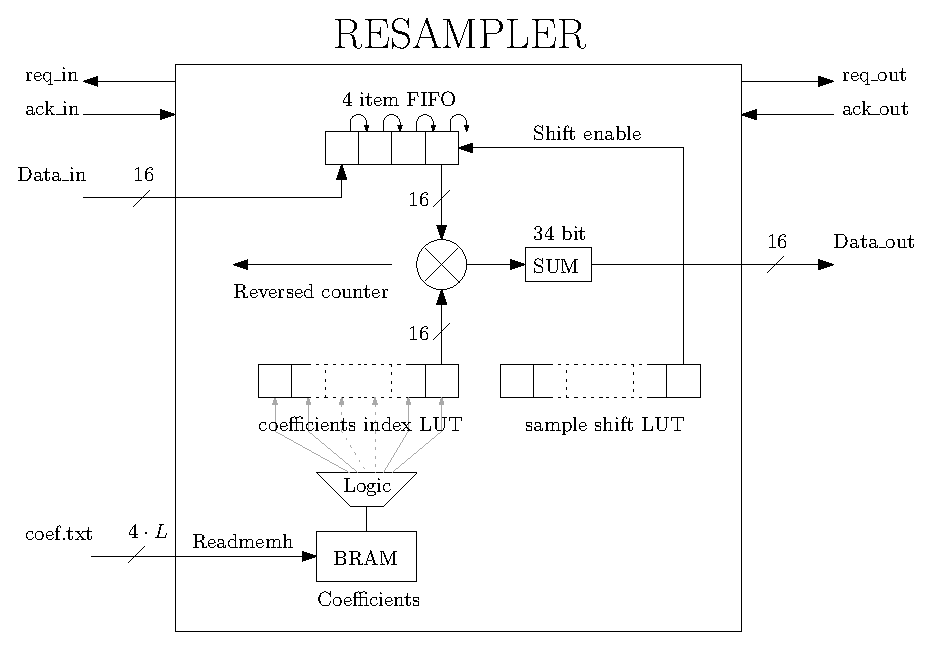
\includegraphics[scale = 0.85]{Images/5_blockdiagram}
    \caption{System overview}
\end{figure}

The resampler is an extension of the implementation of lab 4. The upper part has changed. We can see that four Block RAM modules are used to shift the data samples in.\\

Four DSP units are used to calculated one sample in one cycle. Because of the fact that all these steps are pipelined, we needed to have a stream delay buffer. This stream delay buffer delays the calculated samples one full stream-length minus the additional delay of the calculation pipeline. This ensures that a full stream of samples, is not shifted, but delayed one full stream length.

\newpage
\section{Design choices}

\newpage
\section{Resource usage}
Table~\ref{tab:3ausage} summarizes the resources used by the multi-stream resampler. This list is obtained by running the synthesis step in Xilinx ISE and extracted from the \textit{Summary} and \textit{Device Utilization} report.

\begin{table}[h]
\begin{tabular}{|l|l|l|l|}
\hline
\textbf{Resource} & \textbf{Available} & \textbf{Utilized} & \textbf{Percentage utilized}\\
\hline
Flip Flops	& 54576 & 70 	& 1\%\\
Slice LUTs 	& 27288 & 212 	& 1\%\\
DSP48A1s	& 58 	& 4 	& 6\%\\
BRAM		& 116 	& 2 	& 1\%\\
Bonded IOBs	& 218 	& 38	& 17\%\\
\hline
\end{tabular}
\caption{General resource usage overview}
\label{tab:3ausage}
\end{table} 

4 DSP units are used, since one sample is calculated in one clock cycle, by using the direct form equation.\\

Both the coefficient index and shift enable LUT are stored in DRAM. This because they are both read-only. \\

We tried to use BRAM for our ram modules. They are also shown als Block RAM in our block diagram. However, the compiler has actually not synthesized them as BRAMs but as LUTs. This has probably to do that we did not buffer the output of the RAM, which makes it asynchronous.\\

The compiler did create block ram for the delay buffer. This buffer uses $NR\_STREAMS * DDWIDTH$ bits.

\newpage
\section{System throughput and latency}
The synthesis estimation is as follows:\\

\textit{Minimum period: 6.164ns (Maximum Frequency: 162.234MHz)\\
Minimum input arrival time before clock: 5.080ns\\
Maximum output required time after clock: 3.820ns}\\

After doing the placement and routing step, we get the following timing summary:\\

\textit{Minimum period:   7.528ns{1}   (Maximum frequency: 132.837MHz)\\
Minimum input required time before clock:   4.323ns\\
Maximum output delay after clock:   8.707ns}\\

Since the maximum delay is below 10ns, we can be sure that our design is able to run at 100MHz. Our maximum clock frequency, according to the \textit{Advanced Post-PAR static timing report} under \textit{Timing summary}, is: $\dfrac{1}{8.708ns} \approx 115MHz$. 
   
\newpage
\section{Offline project results}
We managed to get the multiple-stream scaler running on 256 and 512 streams in real-time on the board. With 1024 streams the output audio was noticeably slowed. \\ This likely occurred because we process a few cycles too much before outputting a tap. \\

Next to real-time, we also ran the offline version of the project for 256 and 1024 streams. See Figure~\ref{fig:output} and Figure~\ref{fig:spectrum}.
\begin{figure}[h]
	\centering
	\includegraphics[scale = 0.6]{Images/output_offline.png}
    \caption{Input, and output of 256 and 1024 offline after running on the board.}
    \label{fig:output}
\end{figure}

\newpage

\begin{figure}[h]
	\begin{subfigure}[b]{0.5\textwidth}	
		\includegraphics[scale=0.5]{Images/spectrum_input.png}
		\caption{Input}
	\end{subfigure}
	\begin{subfigure}[b]{0.6\textwidth}	
		\includegraphics[scale=0.5]{Images/spectrum_offline_256.png}
		\caption{Output of offline-256}
	\end{subfigure}
	\begin{subfigure}[b]{0.6\textwidth}	
		\includegraphics[scale=0.5]{Images/spectrum_offline_1024.png}
		\caption{Output of offline-1024}
	\end{subfigure}
	
    \caption{Comparison of the input spectrum and output spectrums.}
    \label{fig:spectrum}
\end{figure}


\clearpage

\newpage
\section{Appendix A: Matlab coefficients script}
\begin{lstlisting}
% Put this in a file named coef_generate_matlab.m, then call it 
% while you are in the file directory. It will write the coefficients
% to the coef.txt file and also return them.

function [y] = coef_generate_matlab(L)
        % make sure that coefficients sum to 1
        y = coef_gen(L);
        y = y/sum(y);

        % quantize and round to nearest integer
        y = y * 160;
        y = round(y*(2^15)); 
             
        % convert to signed int filter coeff
        y = int16(y);
        y = hex(fi(y, 1, 16, 0)); %1 stands for signed, 16 bit out
        
        dlmwrite('coef.txt',y,''); %create file, with no delimiter ''      
end

function [y] = coef_gen(L)
    % generate 4*L coefficients and start at 0 instead of 1 *stupid matlab*
    for n = 1:4*L
            y(n) = lanczos2(((n-1)/L) -2);
    end
end

function y = lanczos2(t)
    if(t <= -2 || t >= 2)
        y = 0;
    else
        y = sinc(t).*sinc(t/2);
    end
end
\end{lstlisting}

Figure~\ref{fig:frq} shows the frequency response of the FIR filter that is generated with help of the matlab code from appendix A.

\begin{figure}[h]
	\includegraphics[scale=0.67]{Images/frequencyplot}
    \caption{Interpolation filter frequency domain (Matlab)}
    \label{fig:frq}
\end{figure}

\newpage
\section{Appendix B: Verilog Code}
File: filter.v.
\begin{lstlisting}[language=Verilog]
`timescale 1ns / 1ps

module filter
       #(parameter DWIDTH = 16,
         parameter DDWIDTH = 2*DWIDTH,
         parameter L = 160,
         parameter L_LOG = 8,
         parameter M = 147,
         parameter M_LOG = 8,
         parameter CWIDTH = 4*L,
         parameter NR_STREAMS = 16,
         parameter NR_STREAMS_LOG = 4)
       (input clk,
        input rst,
        output req_in,
        input ack_in,
        input [0:DWIDTH-1] data_in,
        output req_out,
        input ack_out,
        output [0:DWIDTH-1] data_out);

// Output request register
reg req_out_buf;
assign req_out = req_out_buf;

// Input request register
reg req_in_buf;
assign req_in = req_in_buf;

// Accumulator (assigned to output directly)
reg signed [0:DWIDTH-1] sum;
assign data_out = sum;

// RAM wires and registers
reg ram_enable_buf;
wire ram_enable;
assign ram_enable = ram_enable_buf;

reg [0:NR_STREAMS_LOG-1] ram_address_ptr;
wire [0:NR_STREAMS_LOG-1] ram_address;
assign ram_address = ram_address_ptr;

wire [0:DWIDTH-1] ram_data_out[0:3];
reg signed [0:DWIDTH-1] ram_data_out_buf[0:3];

// input buffer
reg signed [0:DWIDTH-1] data_in_buf;
wire [0:DWIDTH-1] data_in_wire;
assign data_in_wire = data_in_buf;

// Instantiate the RAM modules
rom_mod #(DWIDTH, NR_STREAMS_LOG)
        bram_0 (clk, rst, ram_enable, ram_address, data_in_wire, ram_data_out[0]);
rom_mod #(DWIDTH, NR_STREAMS_LOG)
        bram_1 (clk, rst, ram_enable, ram_address, ram_data_out[0], ram_data_out[1]);
rom_mod #(DWIDTH, NR_STREAMS_LOG)
        bram_2 (clk, rst, ram_enable, ram_address, ram_data_out[1], ram_data_out[2]);
rom_mod #(DWIDTH, NR_STREAMS_LOG)
        bram_3 (clk, rst, ram_enable, ram_address, ram_data_out[2], ram_data_out[3]);

// pipeline stage
reg signed [0:DDWIDTH-1] pl_mul_to_acc_buf[0:3];

// intialize buffers
reg shift_enable;
integer sample_index, buf_ptr;
reg [0:L-1]lookup_shift; //'1' means shift, '0' means no shift
reg signed [0:DWIDTH-1] coef [0:CWIDTH-1], lookup_coefIdx[0:L-1][0:3], coef_preproc[0:3];

reg signed [0:DDWIDTH+1] stream_delay_buf[0:NR_STREAMS-1];


integer i, j;
initial begin
    for(i = 0; i < 4; i = i + 1) begin
        pl_mul_to_acc_buf[i] <= 0;
        ram_data_out_buf[i] <= 0;
    end

    // define shift LUT
    for(i=0;i<L;i=i+1) begin
        if(i*M/L == (i+1)*M/L)
            lookup_shift[i] = 0; //do not shift yet
        else
            lookup_shift[i] = 1; //shift
    end

    // define coef LUT
    for (i = 0; i < L; i = i + 1) begin
        for(j = 0; j < 4; j = j + 1) begin
            lookup_coefIdx[i][j] = j*L + i*M%L;
        end
    end

    for (i = 0; i < NR_STREAMS; i = i + 1) begin
        stream_delay_buf[i] <= 0;
    end

    // import coefficients
    $readmemh("coef.txt", coef, 0, CWIDTH -1);
end

always @(posedge clk) begin
    // Reset => initialize
    if (rst) begin
        req_in_buf <= 0;
        req_out_buf <= 0;
        sum <= 0;
        sample_index <=0;
        buf_ptr <= 0;
        shift_enable <= 0;
        data_in_buf <= 0;
        ram_enable_buf <= 1;
        ram_address_ptr <= 0;
    end
    // !Reset => run
    else begin

        // Read handshake complete
        if (req_in && ack_in) begin
            // shift data in.
            data_in_buf <= data_in;
            ram_enable_buf <= 1;

            req_in_buf <= 0;
        end

        // data shifted in ram
        if (ram_enable_buf== 1) begin
            ram_enable_buf <= 0;
        end

        // Write handshake complete
        if (req_out && ack_out) begin

            // See if we have to shift next stream of samples
            if(ram_address_ptr == NR_STREAMS-1) begin
                shift_enable <= lookup_shift[sample_index];
                sample_index <= (sample_index + 1) % L;
            end

            // if so, ask for new input data
            if(shift_enable == 1) begin
                req_in_buf <= 1;
            end
            else begin
                // do NOT ask for new input data, re-use buffered data (stream_delay_buf)
            end
            req_out_buf <= 0;
        end

        // Processing state
        if (!req_in && !ack_in && !req_out && !ack_out && ram_enable_buf == 0) begin

            //retrieve samples
            ram_data_out_buf[0] <= ram_data_out[0];
            ram_data_out_buf[1] <= ram_data_out[1];
            ram_data_out_buf[2] <= ram_data_out[2];
            ram_data_out_buf[3] <= ram_data_out[3];

            //multiply with coefficients
            pl_mul_to_acc_buf[0] <= ram_data_out_buf[0]*coef_preproc[0];
            pl_mul_to_acc_buf[1] <= ram_data_out_buf[1]*coef_preproc[1];
            pl_mul_to_acc_buf[2] <= ram_data_out_buf[2]*coef_preproc[2];
            pl_mul_to_acc_buf[3] <= ram_data_out_buf[3]*coef_preproc[3];

            //accumulate and put into delay buffer
            stream_delay_buf[buf_ptr]	<= 	pl_mul_to_acc_buf[0] +
                            pl_mul_to_acc_buf[1] +
                            pl_mul_to_acc_buf[2] +
                            pl_mul_to_acc_buf[3];

            // increment pointers
            ram_address_ptr <= (ram_address_ptr + 1) % NR_STREAMS;
            buf_ptr <= (buf_ptr + 1)%((NR_STREAMS));

            // output data (+2 offset is the delay of the pipeline)
            sum <= stream_delay_buf[(buf_ptr+2)%NR_STREAMS][3:DWIDTH+2];

            // preprocess next coefficients
            coef_preproc[0] <= coef[lookup_coefIdx[sample_index][0]];
            coef_preproc[1] <= coef[lookup_coefIdx[sample_index][1]];
            coef_preproc[2] <= coef[lookup_coefIdx[sample_index][2]];
            coef_preproc[3] <= coef[lookup_coefIdx[sample_index][3]];

            // request output
            req_out_buf <= 1;
        end

    end
end

endmodule
\end{lstlisting}

\newpage

File: bram$\_$mod.v.
\begin{lstlisting}[language=Verilog]
`timescale 1ns / 1ps
module rom_mod
       #(parameter RAM_WIDTH = 16,
         parameter RAM_ADDR_BITS = 10 )(
           input clk,
           input rst,
           input enable,
           input [0:RAM_ADDR_BITS-1] ram_address,
           input [0:RAM_WIDTH-1] in_data,
           output [0:RAM_WIDTH-1] out_data);

(* RAM_STYLE="block" *)
reg [RAM_WIDTH-1:0] bram [(2**RAM_ADDR_BITS)-1:0];
wire [RAM_ADDR_BITS-1:0] ram_address_ptr;

// output buffer
//reg [0:RAM_WIDTH-1] data_out_buf;
assign out_data = bram[ram_address_ptr];

// reverse all address wires
generate
    genvar j;
for(j=0;j<RAM_ADDR_BITS;j=j+1) begin: reverse
    assign ram_address_ptr[j] = ram_address[j];
end
endgenerate

    integer i;
initial begin
    for(i=0;i<2**RAM_ADDR_BITS-1;i=i+1)
        bram[i] <= 0;
end

always @(posedge clk) begin
    if(rst) begin
        //data_out_buf <= 0;
    end
    else begin
        if (enable) begin
            bram[ram_address_ptr] <= in_data;
        end
        //data_out_buf <= bram[ram_rd_address];
    end
end
endmodule
\end{lstlisting}

\end{document}
